\documentclass{article}
\usepackage{amsmath}
\usepackage{amssymb}
\usepackage{graphicx}
\usepackage[margin=1in]{geometry}
\usepackage{hyperref}
\usepackage{caption}
\usepackage{float}
\graphicspath{{images/}}
\hypersetup{
  colorlinks=true,
  urlcolor=blue,
}
\begin{document}

\title{Notes on the Plastic Ratio}
\author{Aresh Pourkavoos}
\maketitle

The plastic ratio $\rho$ is the real solution to $\rho^3 = \rho+1$,
with an approximate value of $1.3247$.
Its definition puts it into the set of numbers
that gives the golden ratio many of its interesting
(and, to some, mystical) properties: the algebraic integers.
A few quick facts:
\begin{itemize}
\item
  Contrary to first impressions,
  the word ``plastic'' in this constant's name
  refers not to the material but to the idea of plasticity, or flexibility.
\item
  It is the smallest of the PV numbers,
  which are the reals greater than 1
  whose powers approach integers.
  The powers of $\rho$ approach a sequence known as the Perrin numbers.
  (The golden ratio is also a PV number,
  and its powers approach the Lucas numbers,
  which are closely related to the Fibonacci numbers.)
\end{itemize}

Being an algebraic number,
the plastic ratio can be used to ``extend'' the rational numbers
to create a new field,
a set of numbers that can be added, subtracted, multiplied, and divided
in the same way as the rational, real, or complex numbers.
Since $\rho$ itself is included in this field,
so must $b\rho$ for all rational numbers $b$,
since the field is closed under multiplication.
Likewise, it must be possible to add any rational number $a$
to get a new element,
so all numbers of the form $a+b\rho$ are also elements of this field.
They are also all unique,
since if there were two different choices of $a$ and $b$
that led to the same number,
it would imply that $\rho$ is rational.
However, the field is still not complete
because $\rho^2$ needs to be in it
(multiplying $\rho$ by itself),
but it cannot be expressed as $a+b\rho$
for any rational $a$ and $b$,
since that would imply that $\rho$ is the solution to a quadratic equation
rather than a cubic one.
Thus all numbers of the form $a+b\rho+c\rho^2$
for rational $a$, $b$, and $c$ should be part of this field.
However, the pattern stops at $\rho^3$,
since $\rho^3=\rho+1$,
so it is already in the field thus far.
In fact, it is always possible to add, subtract, multiply, and divide
within $a+b\rho+c\rho^2$ and remain within the set.

A number of the form $a+b\rho+c\rho^2$
may be considered as a vector in 3D
whose coordinates are rational numbers.
Addition and subtraction are performed elementwise,
so they act like addition and subtraction of vectors.
Multiplying by a rational number scales the whole vector.
However, it is not generally possible to multiply two vectors,
but it is possible to multiply two elements of the plastic field
to obtain another element.
Moreover, multiplying by a vector is a linear transformation of 3D space,
i.e. it can be represented by a matrix
\begin{align*}
  a+b\rho+c\rho^2 &\cong
  \begin{bmatrix}
    a & c & b \\
    b & a+c & b+c \\
    c & b & a+c
  \end{bmatrix} = M. \\
\end{align*}
The columns of the matrix correspond to the components of
$a+b\rho+c\rho^2$ after multiplication by 1, $\rho$, and $\rho^2$, respectively.
While multiplying numbers of this form is easy to do by hand
using the distributive property and reducing $\rho^3$ to $1+\rho$
(and $\rho^4$ to $\rho+\rho^2$),
it is not obvious how to divide two of these numbers,
i.e. to find the multiplicative inverse of one of them.
However, the matrix form provides a path forward:
inverting the corresponding matrix should give a new matrix
corresponding to the inverse of the number,
and luckily, computing the inverse of a matrix is a well-known process.
\begin{align*}
  M^{-1} &= \frac{\mathrm{adj}(M)}{\lvert M \rvert} \\
  \mathrm{adj(M)} &=
  \begin{bmatrix}
    d & \\
    e & \hdots \\
    f &
  \end{bmatrix}
  \cong d+e\rho+f\rho^2 \\
  d &=
  %% \begin{vmatrix}
  %%   a+c & b+c \\
  %%   b & a+c
  %% \end{vmatrix} =
  (a+c)^2-b(b+c) \\
  e &=
  %% \begin{vmatrix}
  %%   b+c & b \\
  %%   a+c & c
  %% \end{vmatrix} =
  c^2-ab \\
  f &=
  %% \begin{vmatrix}
  %%   b & a+c \\
  %%   c & b
  %% \end{vmatrix} =
  b^2-(a+c)c \\
  \lvert M \rvert &= ad+ce+bf \\
  \frac{\lvert M \rvert}{a+b\rho+c\rho^2}
  &= d+e\rho+f\rho^2 \\
  &= (a+b\rho_2+c\rho_2^2)(a+b\rho_3+c\rho_3^2) \\
  &= \frac{1}{4}\left((2a-b\rho+c(2-\rho^2))^2+(b-c\rho)^2(3\rho^2-4)\right) \\
  &= K \\
  a, b, c \in \mathbb{R}: & K \geq 0, \\
  & K = 0 \iff a\rho^2 = b = c\rho \\
  a, b, c \in \mathbb{Q}: & K = 0 \iff a = b = c = 0, \\
  & \mathrm{sgn}(\lvert M \rvert) = \mathrm{sgn}(a+b\rho+c\rho^2) \\
\end{align*}

My most recent encounter with this number
came from the uniform polyhedron known as
the snub icosidodecadodecahedron, or ``sided'' for short.

\begin{center}
  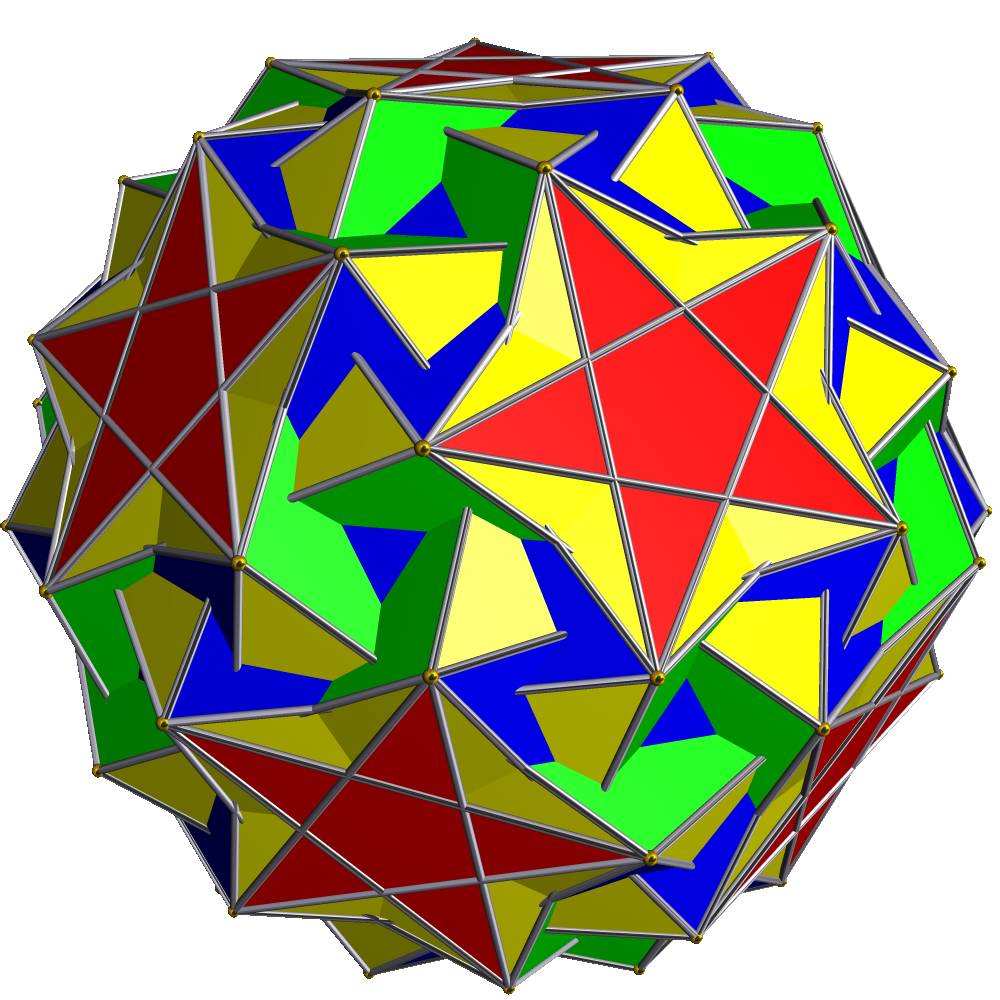
\includegraphics[width=0.25\linewidth]{sided.png} \\
  Created using \href{http://www.software3d.com/Stella.php}{Stella}
\end{center}

Like many polyhedra related to the icosahedron,
the coordinates of its vertices involve the golden ratio.
What surprised to me, however,
was the inclusion of the plastic ratio as well,
which does not appear in any other uniform polyhedra.
At a certain scale, its vertices may be written as follows,
where $\varphi$ is the golden ratio:

\begin{align*}
  & (2\alpha, 2\beta, 2\gamma), \\
  & (\alpha+\beta/\varphi+\gamma\varphi,
  -\alpha\varphi+\beta+\gamma/\varphi,
  \alpha/\varphi+\beta\varphi-\gamma), \\
  & (-\alpha/\varphi+\beta\varphi+\gamma,
  -\alpha+\beta/\varphi-\gamma\varphi,
  \alpha\varphi+\beta-\gamma/\varphi), \\
  & (-\alpha/\varphi+\beta\varphi-\gamma,
  \alpha-\beta/\varphi-\gamma\varphi,
  \alpha\varphi+\beta+\gamma/\varphi), \\
  & (\alpha+\beta/\varphi-\gamma\varphi,
  \alpha\varphi-\beta+\gamma/\varphi,
  \alpha/\varphi+\beta\varphi+\gamma),
\end{align*}
where
\begin{align*}
  \alpha &= \rho+1, \\
  \beta &= \varphi^2(\rho^2+\rho)+\varphi, \\
  \gamma &= \rho(\varphi+\rho).
\end{align*}

These 5 sets of coordinates form a single pentagrammic face of sided.
The 3 coordinates of each vertex are rotated to create 10 new triplets,
e.g. $(2\alpha, 2\beta, 2\gamma)$ yields
$(2\beta, 2\gamma, 2\alpha)$ and $(2\gamma, 2\alpha, 2\beta)$.
This represents a 120-degree rotation about the axis $x=y=z$,
and the image above is almost looking down on such a threefold symmetry axis,
running through the center of 3 pentagrams.
Next, even sign changes are applied,
meaning that that the 4 possible ways of negating none or two of the coordinates
represent vertices of sided,
bringing the total from 15 to 60, the actual number of vertices.
The even sign changes represent 180-degree rotations,
and the twofold symmetry axes around which these rotations are performed
may also be seen above, running between adjacent pentagrams.

In the plastic ratio base,
the only digits are zero and one since $\rho < 2$,
and all ones must have at least 4 zeros between them.
This is because a pair of ones with 3 zeroes between them
would be $1+\rho^4=\rho^5$ (times some power of $\rho$ overall),
and any closer ones would also carry over into the next power of $\rho$
(or even the one after that).
The carryover rules are as follows:
\begin{center}
  \begin{tabular}{|c|c|c|c|c|}
    \hline
    010001 & 0100100000 & 0101000 & 0011 & 00200000 \\ \hline
    100000 & 1000000001 & 1000001 & 1000 & 10000001 \\ \hline  
  \end{tabular}
\end{center}
The integer place values are 1, 2, 3, 4, 5, 6, 8, 11, 15, 20, 25, 31, $\ldots$,
where $P_n=n+1$ for $n=0, \ldots, 4$ and $P_{n+5}=P_n+P_{n+4}$.
It follows the same constraints as the real base,
and in fact produces all terminating sequences that follow these constraints
(with a finite number of 1s) in lexicographical order.

\end{document}
